% !TEX root = macfp_2017_gasphase.tex

\subsection{Case 3: Turbulent Pool Fires with Liquid Fuel} \label{sec:liquid_pool_fires}

\subsubsection{Experiment}

The liquid pool fire experiment selected for the first MaCFP workshop is a 0.305-m diameter methanol pool fire previously studied at the University of Waterloo (UW)~\cite{Case3_EXP_1,Case3_EXP_2}. The UW flame was established over a modified liquid pan burner designed for free air entrainment. The burner was operated at steady state with a gravity fuel feed of 1.35~cm$^3$/s (1.07 g/s) for a total heat release rate of 22.6~kW. The height of the burner lip above the liquid fuel surface was 1~cm. The flame was approximately 0.5-m-high and featured a strong puffing instability; the frequency of oscillation was 2.8~Hz.

Time-resolved velocity (using two component, forward-scatter Laser Doppler Anemometry) and temperature (using 50~micron diameter, bare-wire Pt-Pt-10\%Rh thermocouples with 75-100~micron beads) were measured in the highly-fluctuating region of the flame, $i.e.$ up to radial positions located 16~cm from the pool fire centerline and up to 30~cm vertical elevation. Direct and Schlieren photography of the luminous flame were used to characterize the macroscopic and oscillatory behavior of the flame.

Time series of data were ensemble-averaged to provide mean and {\it rms} values as well as correlation coefficients~\cite{Case3_EXP_2}. Errors in mean and {\it rms} velocities and mean temperatures were estimated as $\pm$5\% at 95\% confidence; errors in Reynolds stresses were estimated as $\pm$15\% at 95\% confidence~\cite{Case3_EXP_1}. Errors in {\it rms} temperatures and velocity-temperature correlations were difficult to estimate and were not quantified. No correction was made to temperature measurements for radiation or catalytic effects (estimated to be less than 5\%).

\subsubsection{Simulations}

Three groups submitted computational results for Case 3: UGent~\cite{Case3_SIM_UGent}, UMD~\cite{Case3_SIM_UMD} and VTT~\cite{Case3_SIM_VTT}. UGent used FireFOAM version 2.2.x~\cite{FireFOAM}; UMD used a shared development version of FireFOAM (FireFOAM-dev)~\cite{FireFOAM}; VTT used an official release of FDS (version 6.5.3)~\cite{FDS}.

Two specific challenges were found in the design of a computational grid for LES simulations of the UW pool fire experiment. The first challenge is to provide suitable grid resolution to capture the intermittent boundary layer flame and thermals that result from the puffing instability. As discussed in section~\ref{sec:CGD}, this requires millimeter-scale resolution. The second challenge is the presence of a 1-cm-high pool lip in the UW experiment. The presence of the lip leads to complex flow patterns close to the edges of the methanol pool surface that also require millimeter-scale resolution to be correctly captured by the computational grid.

The computational groups responded to these two challenges in different ways: UGent adopted a 5-mm resolution in the flame zone (both in the horizontal and vertical directions) and included the burner lip in the numerical configuration; UMD adopted a 2.5-mm resolution in the vertical direction but also used a coarser 10-mm resolution in the horizontal directions and did not account for the presence of the lip; VTT adopted a 2.5-mm resolution (both in the horizontal and vertical directions) and did not account for the presence of the lip.

An important difference in the numerical treatment of the UW experiment is that while UGent and UMD prescribed the fuel evaporation rate using the measured mean experimental value (1.07 g/s), VTT adopted a more ambitious treatment in which the fuel evaporation rate is calculated as a function of the gas-to-liquid thermal feedback. In the simulation performed by VTT, the fuel evaporation rate is under-predicted by a factor close to 1.7 leading to a flame size of 13 kW (compared to 22 kW in simulations by UGent and UMD).

\begin{figure}
\centering
(a)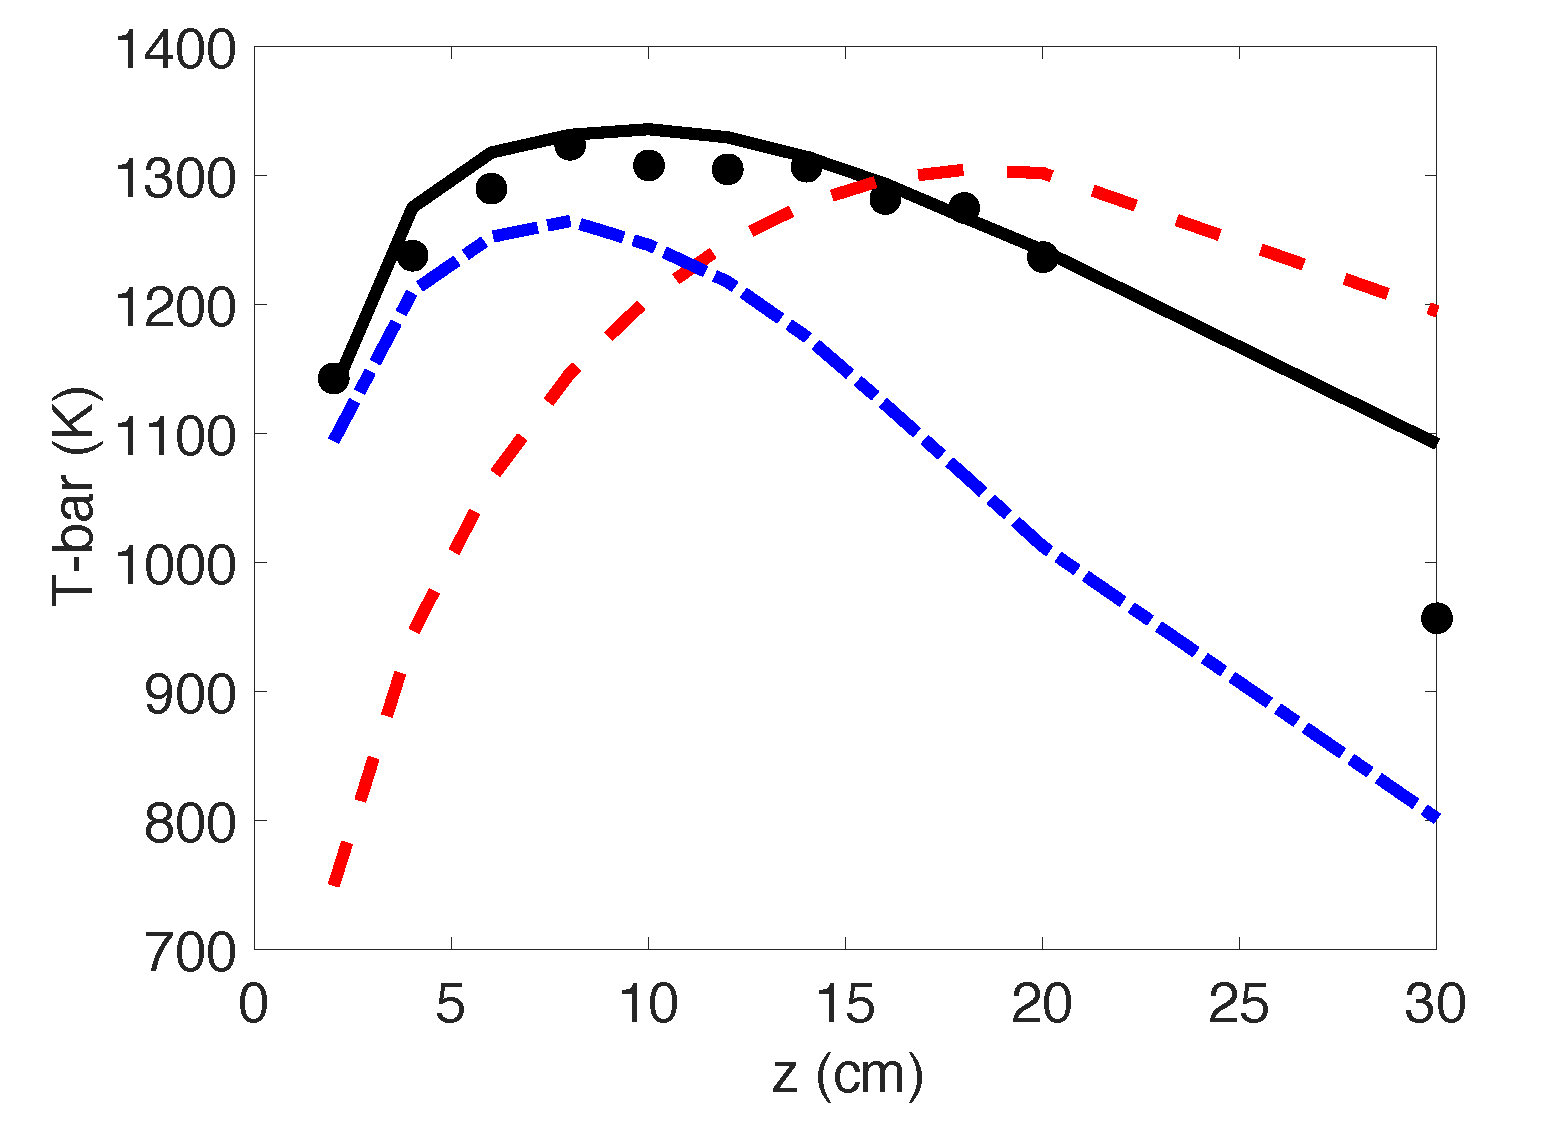
\includegraphics[height=2.2in]{Figures/Case3-Fig1a.png}
(b)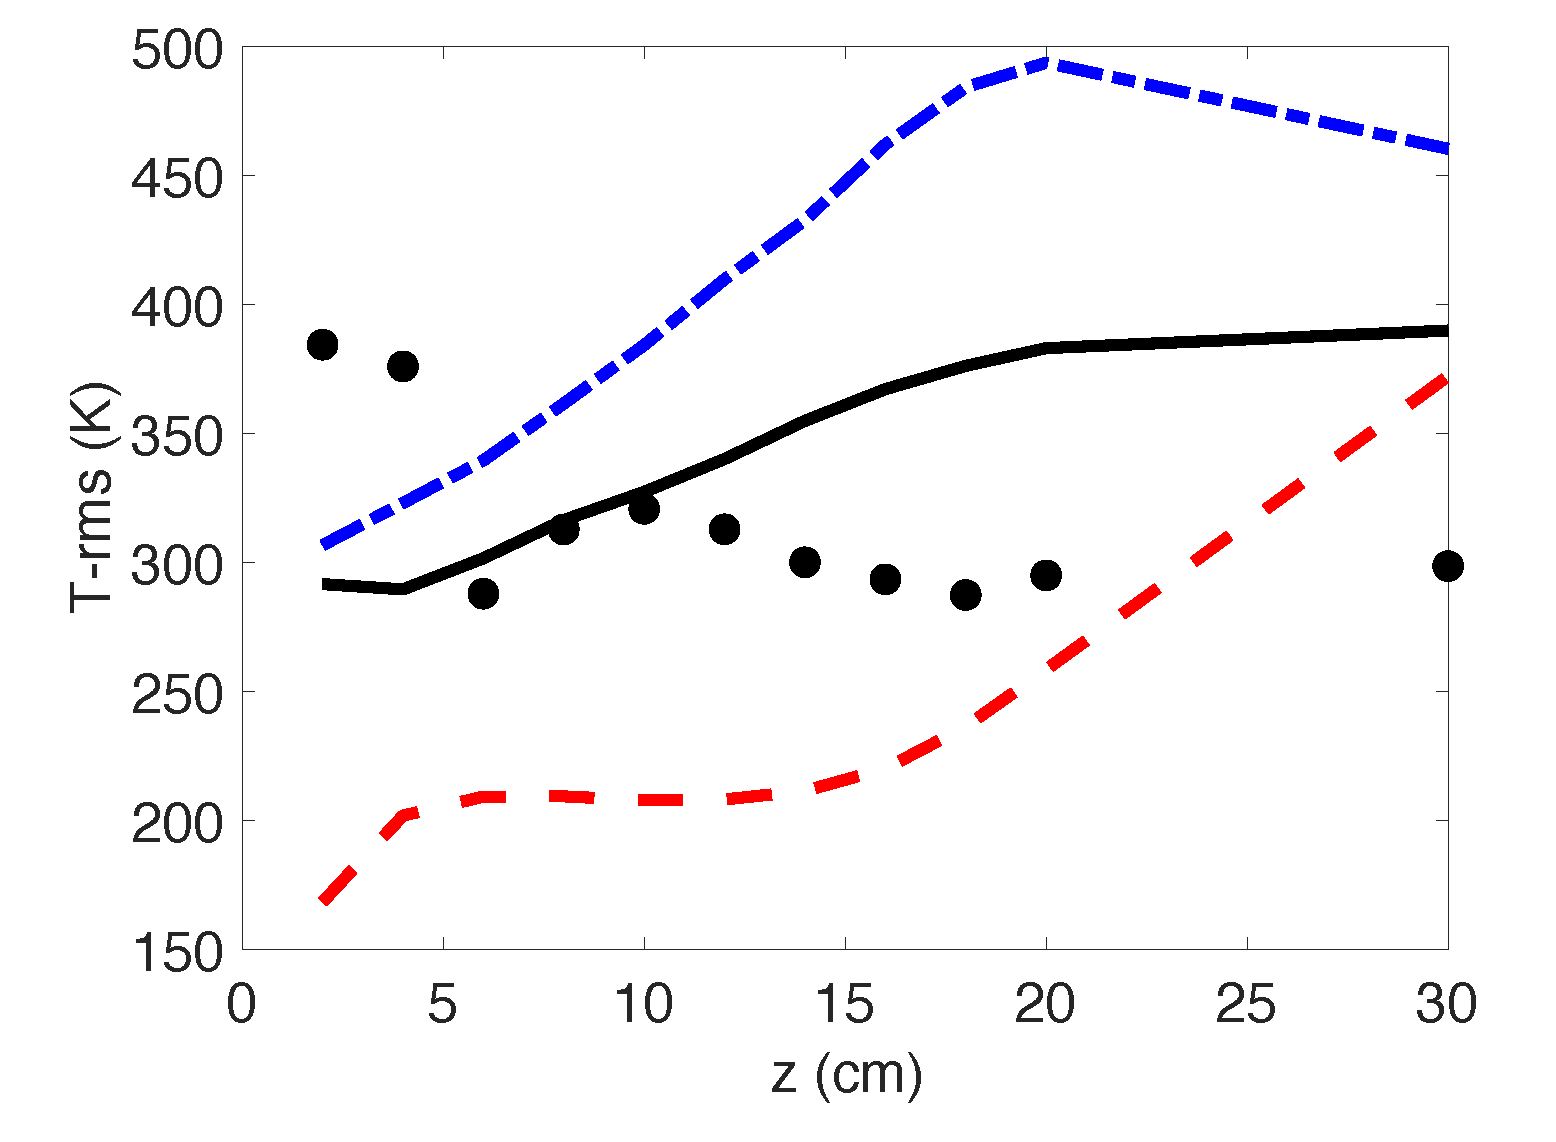
\includegraphics[height=2.2in]{Figures/Case3-Fig1b.png}
(c)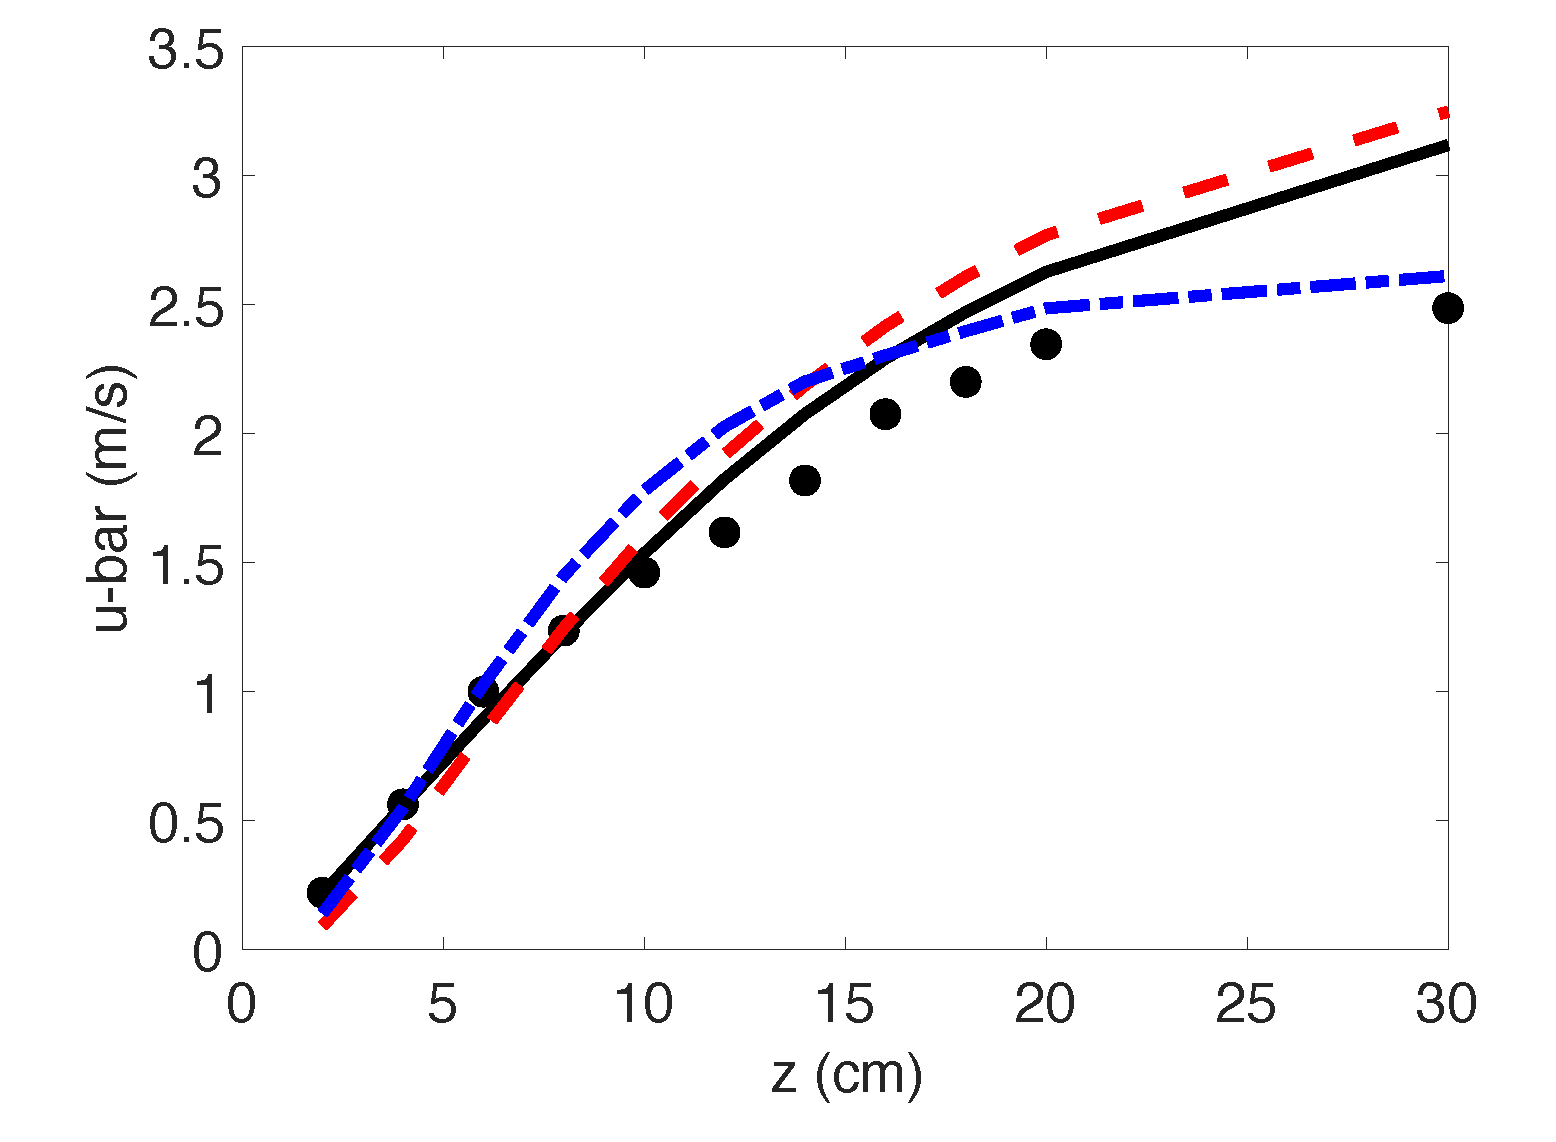
\includegraphics[height=2.2in]{Figures/Case3-Fig1c.png}
(d)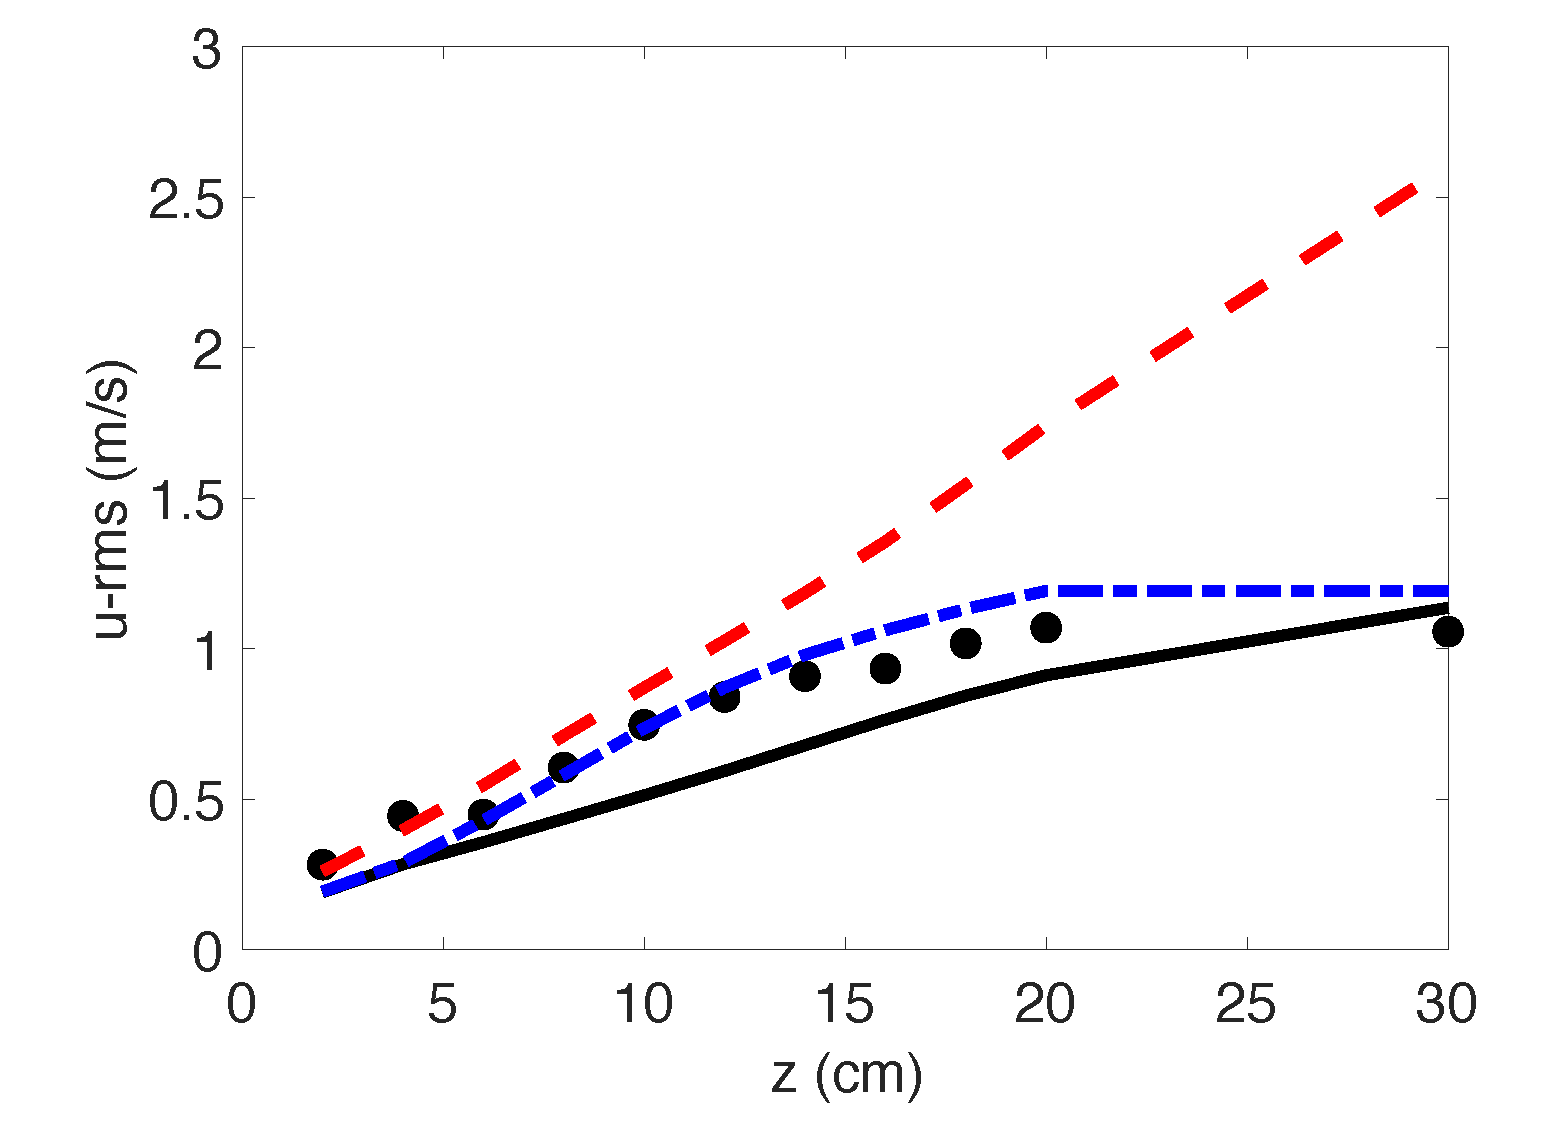
\includegraphics[height=2.2in]{Figures/Case3-Fig1d.png}
\caption{Case 3. Vertical variations along the pool centerline: (a) mean temperature; (b) {\it rms} temperature; (c) mean vertical velocity; (d) {\it rms} vertical velocity. Comparison between experimental data (black circles) and numerical results from UGent (black solid line), UMD (red dashed line), VTT (blue dash-dotted line).}
\label{fig:Case3-Fig1}
\end{figure}

Additional differences in the numerical treatment of the UW experiment include differences in the choice of physical models (see section~\ref{sec:PM} for details on baseline choices). UGent deviated from baseline choices in FireFOAM and used the dynamic Smagorinsky model~\cite{Moin:1991} for subgrid-scale turbulence, the Eddy Dissipation Concept (EDC) model~\cite{Magnussen:1981} for combustion, and an emission/absorption treatment of the RTE for radiation combined with a Weighted-Sum-of-Gray-Gases model~\cite{Dorigon:2013} for gas radiation (the global radiative loss fraction was predicted to be equal to 16.4\%, a value that is close to the empirically-determined value of 17-18\%); in the solution of the RTE, the discretization of angular space used 72 angles. UMD used the baseline configuration of FireFOAM; the value of the global radiative loss fraction was prescribed as equal to 18\%; in the solution of the RTE, the discretization of angular space used 16 angles. VTT used the baseline configuration of FDS: the values of the global radiative loss fraction was prescribed as equal to 17\%; in the solution of the RTE, the discretization of angular space used 104 angles.

\begin{figure}
\centering
(a)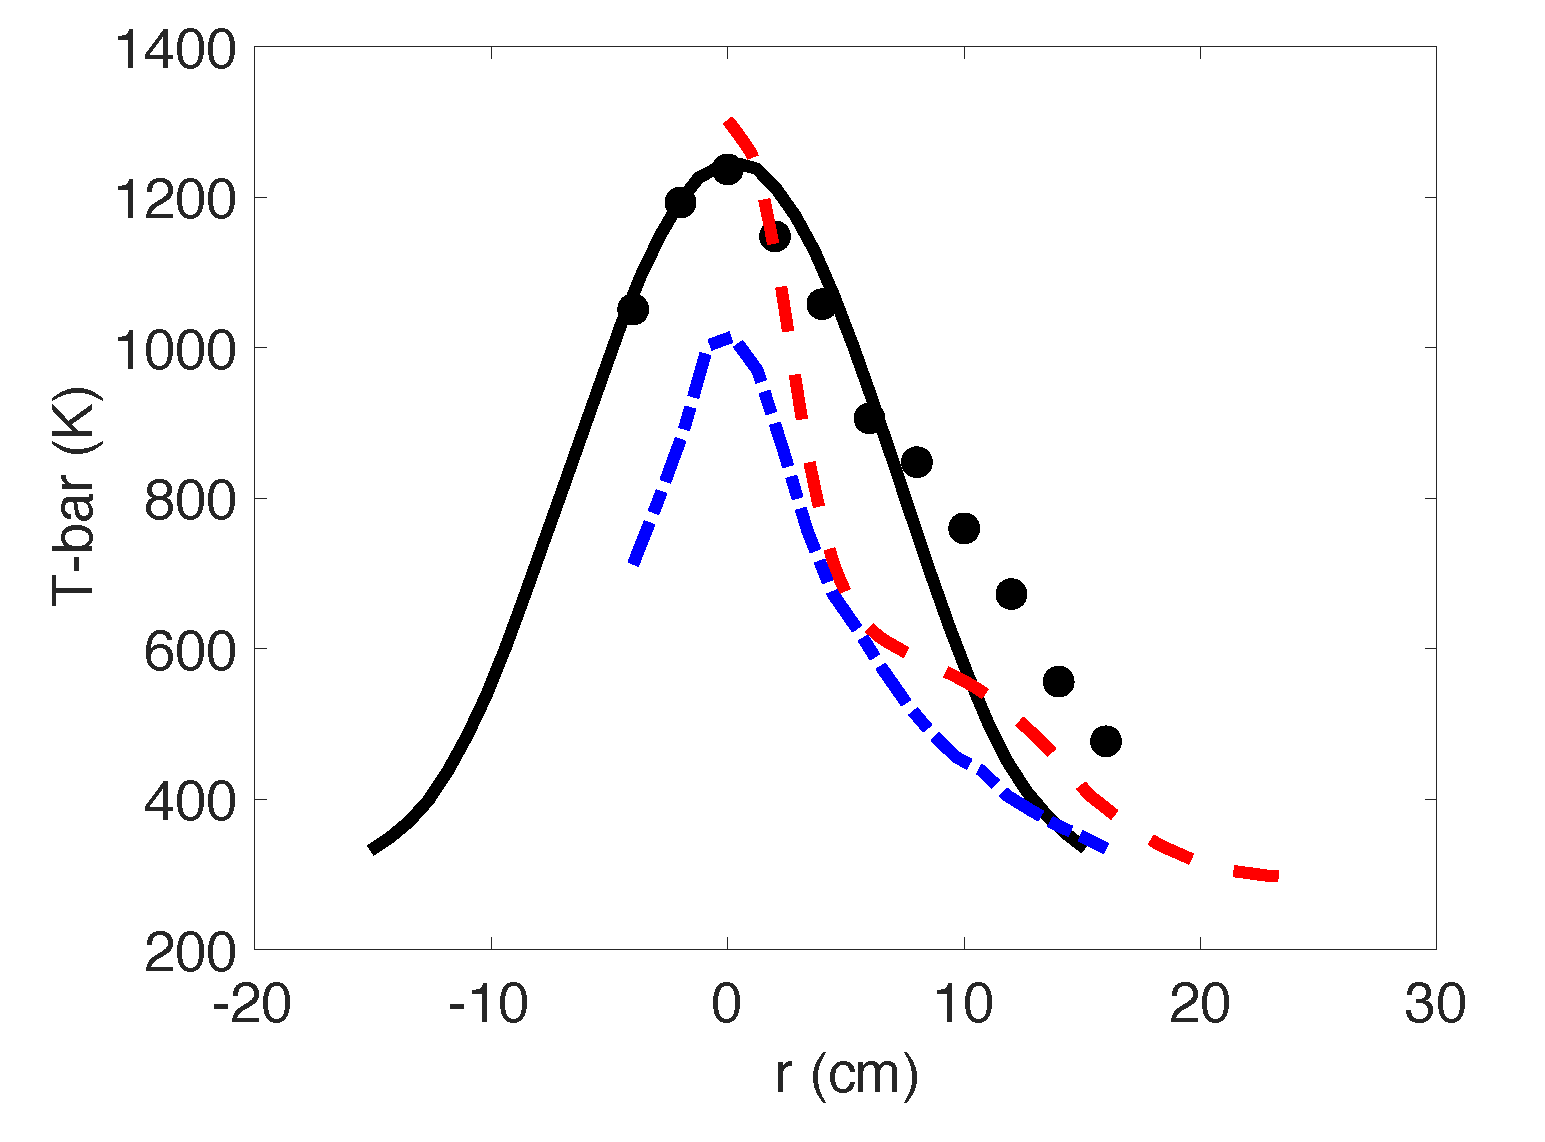
\includegraphics[height=2.2in]{Figures/Case3-Fig2a.png}
(b)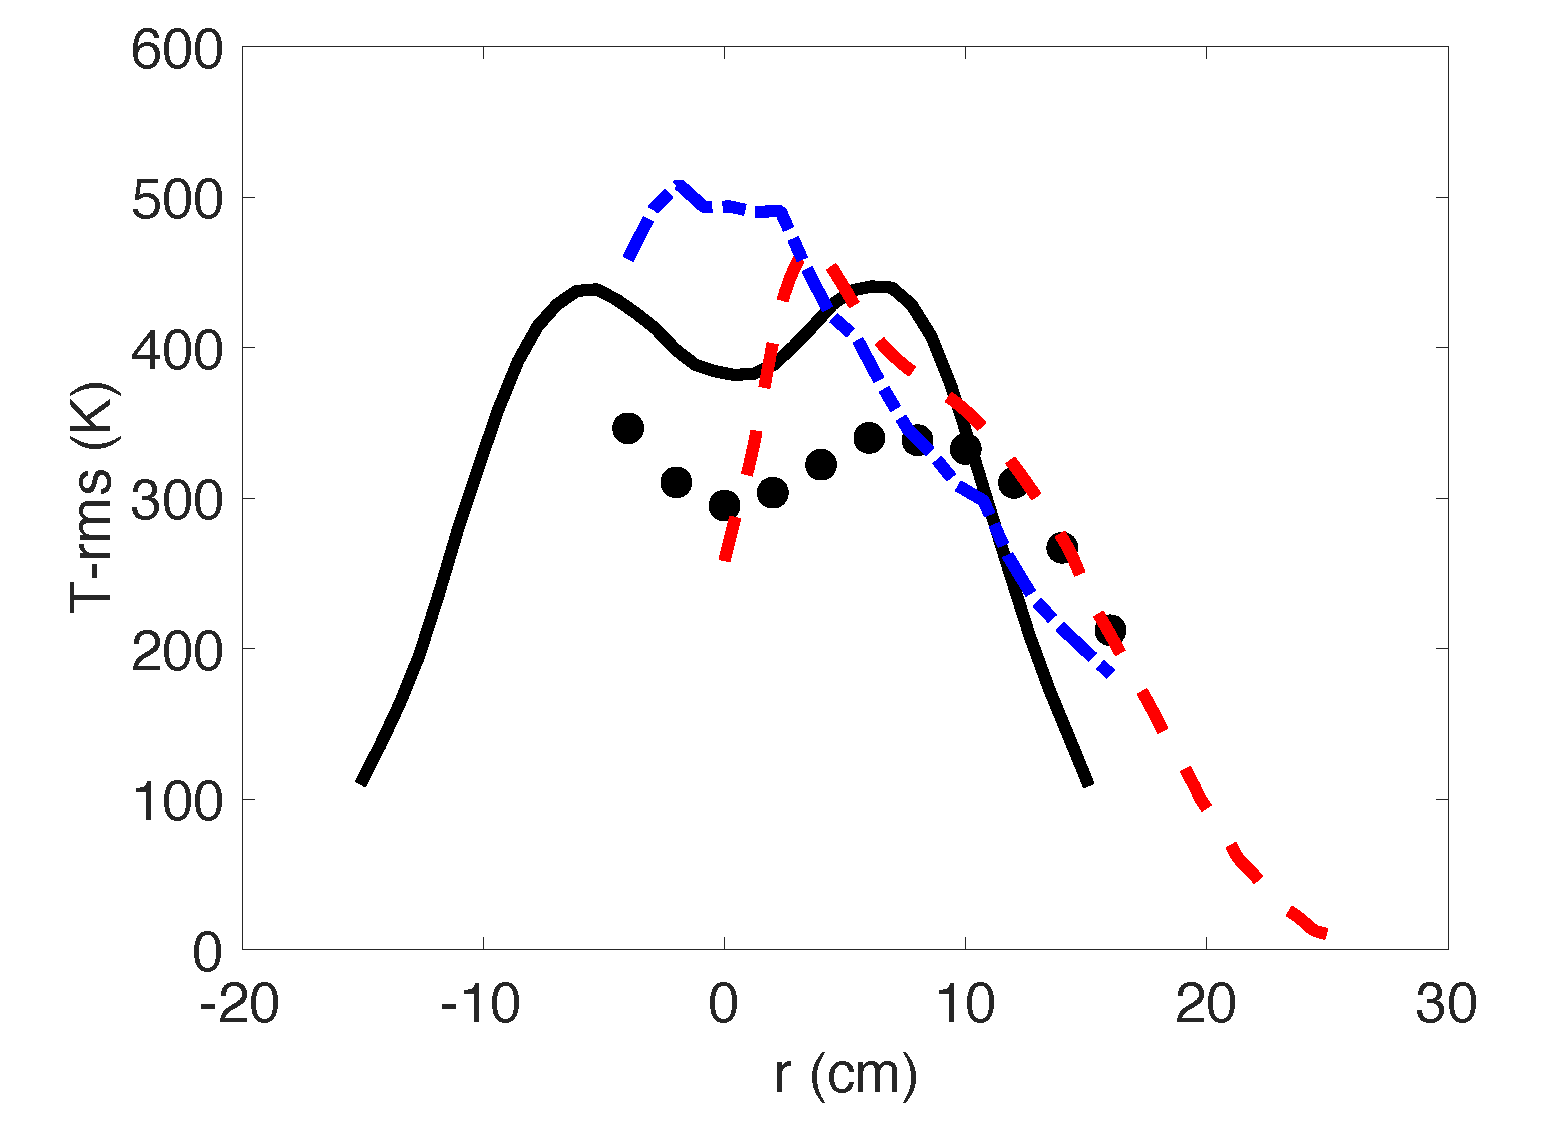
\includegraphics[height=2.2in]{Figures/Case3-Fig2b.png}
(c)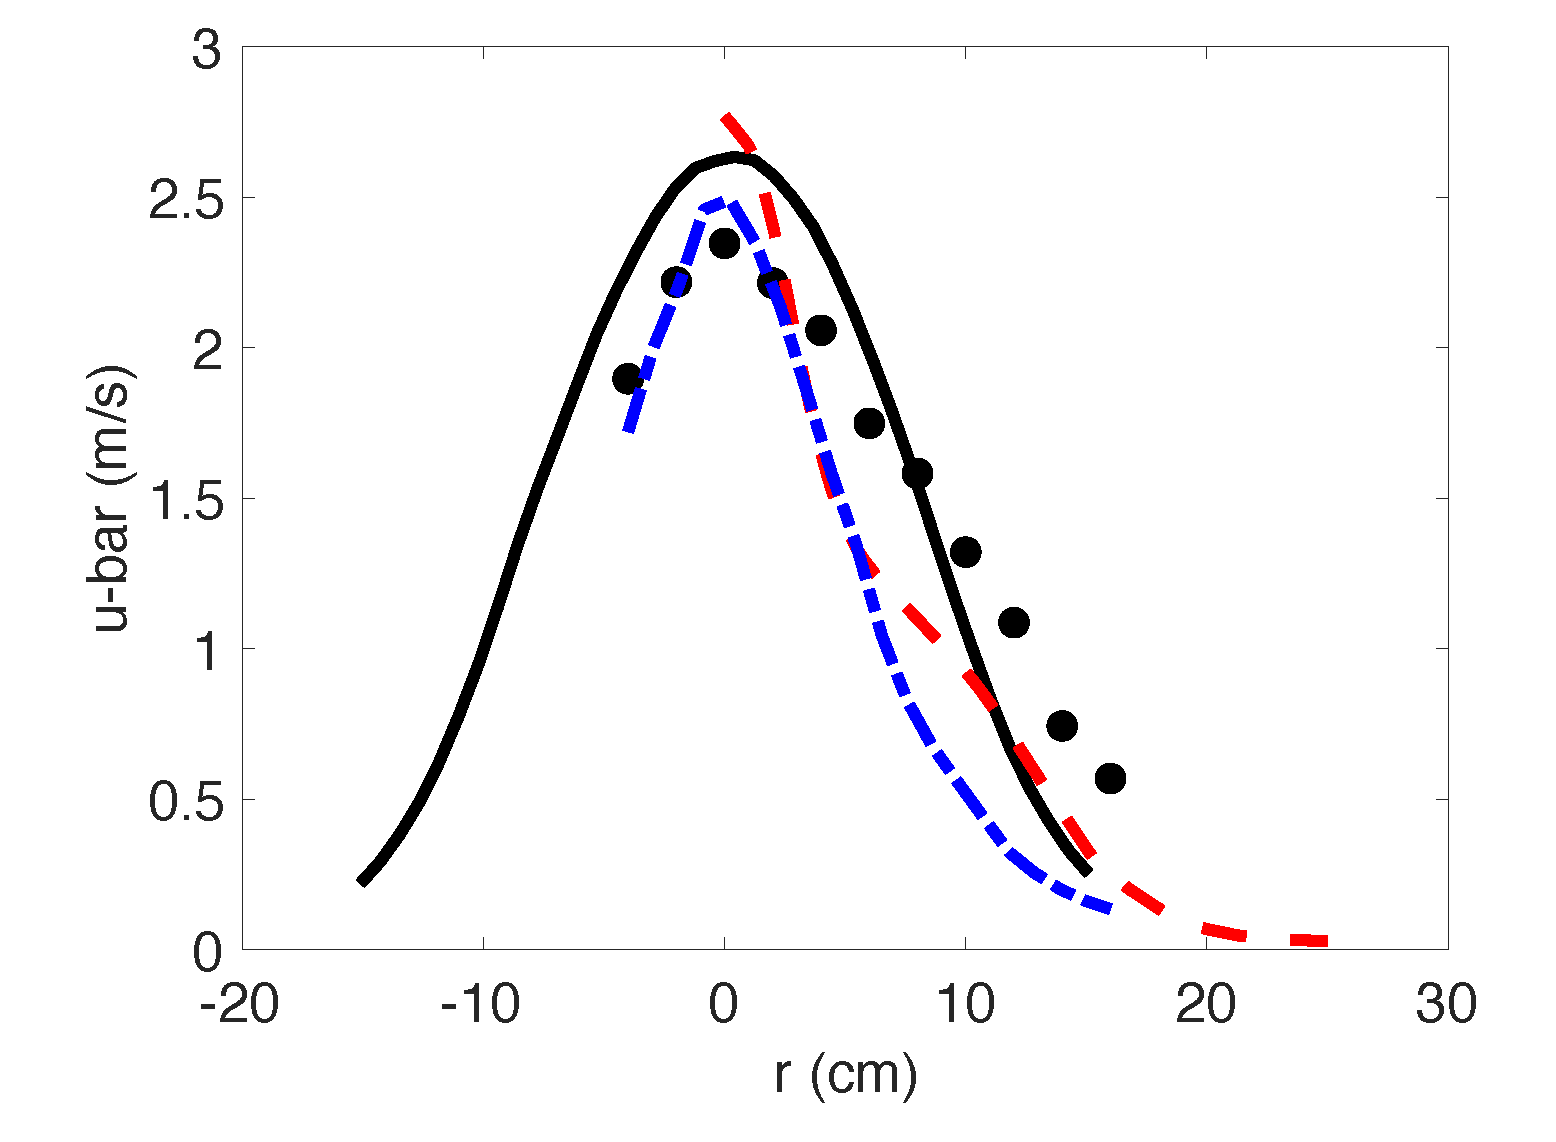
\includegraphics[height=2.2in]{Figures/Case3-Fig2c.png}
(d)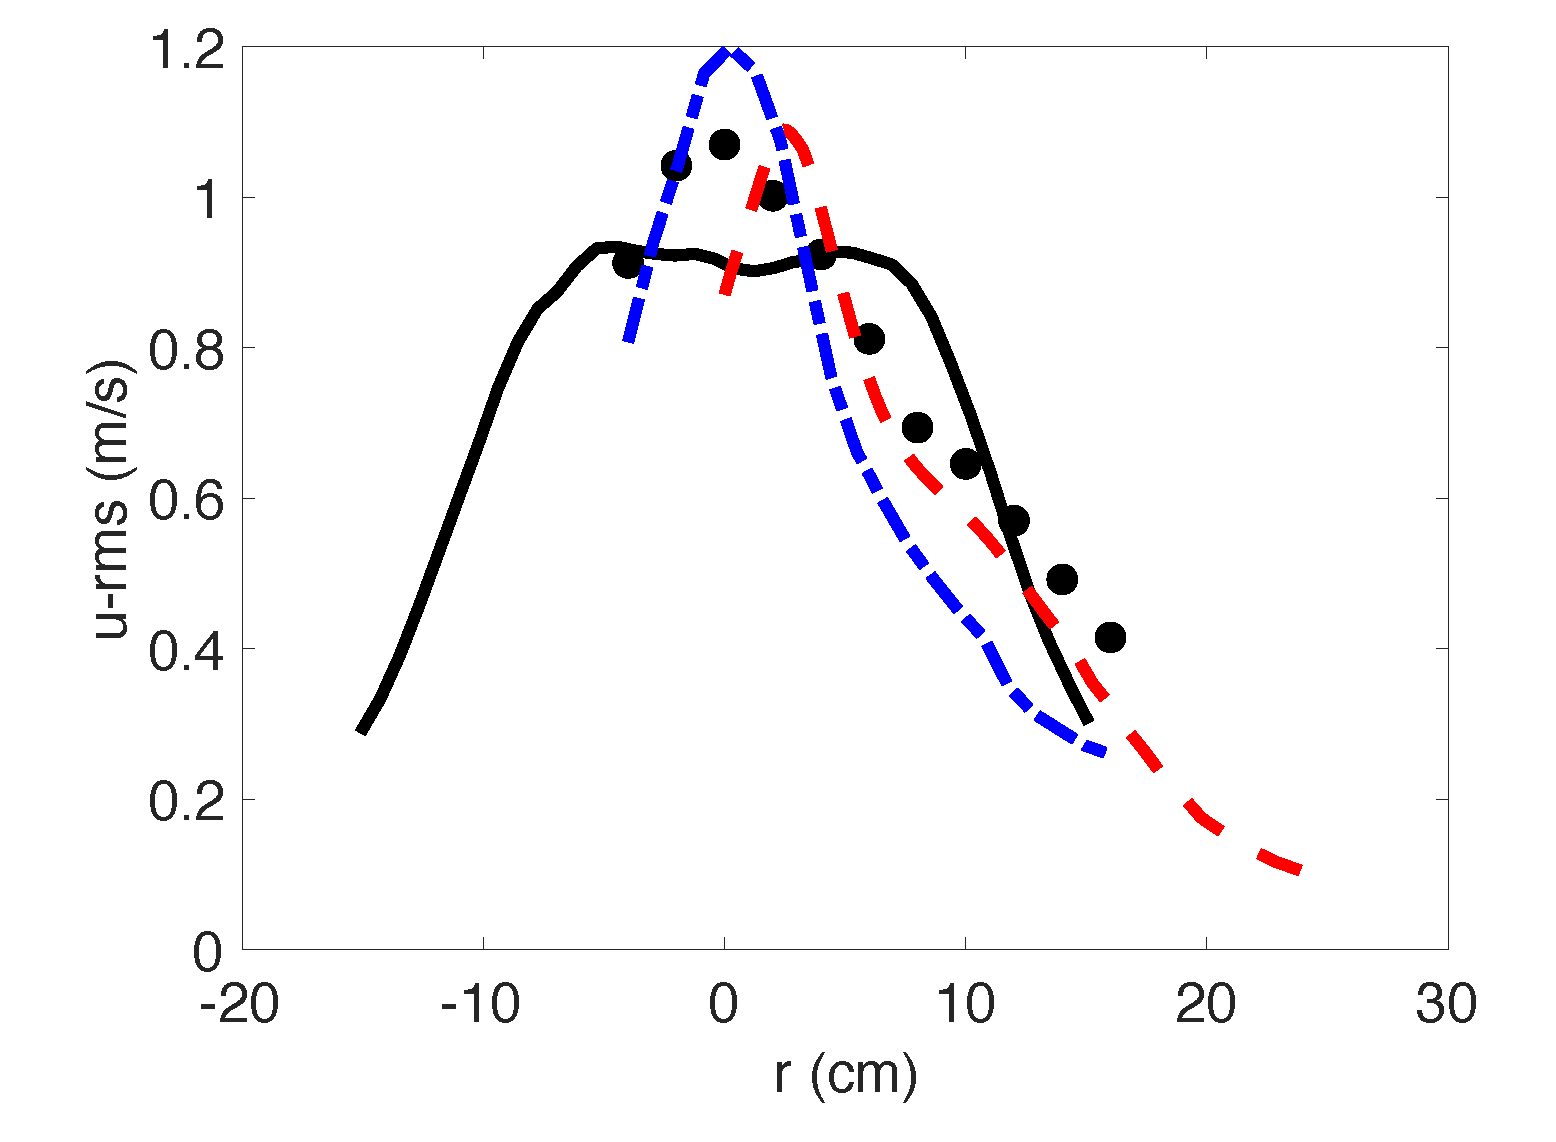
\includegraphics[height=2.2in]{Figures/Case3-Fig2d.png}
\caption{Case 3. Radial variations at elevation $z$ = 20~cm: (a) mean temperature; (b) {\it rms} temperature; (c) mean vertical velocity; (d) {\it rms} vertical velocity. See caption of Fig.~\ref{fig:Case3-Fig1}.}
\label{fig:Case3-Fig2}
\end{figure}

\subsubsection{Summary}

All simulations correctly reproduce a pulsating flame with a frequency of oscillation close to the measured value (2.8 Hz): 2.8 Hz (UGent), 2.2 Hz (UMD), 3 Hz (VTT). Figures~\ref{fig:Case3-Fig1} and~\ref{fig:Case3-Fig2} present a small representative sample of comparisons between experimental data and numerical simulations. Additional comparisons can be found in~\cite{MaCFP_wks_presentations}. Overall, the UGent simulation shows good agreement with experimental data and provides a satisfactory description of the flame structure. The accuracy of the UMD simulation is limited by insufficient grid resolution. The accuracy of the VTT simulation is limited by an inaccurate prediction of the total heat release rate.

It is worth emphasizing that the experimental database describing the UW methanol pool fire experiment is quite unique because it not only contains data on first and second-order statistical moments of temperature and vertical/radial velocities, but also contains data on Reynolds shear stresses and turbulent heat fluxes~\cite{Case3_EXP_1,Case3_EXP_2}. There are also some limitations in the database that are worth pointing out for future studies: (1) the UW database is limited to the flame near-field, $i.e.$ to low elevations ($z \leq 30$~cm), and there is a need to provide data over the full flame region ($0 \leq z \leq L_f$, where $L_f$ is the flame height; $L_f  \approx 0.5$~m in the UW experiment); (2) the flame is only weakly turbulent and there is a need to provide data for larger flame sizes, $i.e.$ for larger pool diameters ($D \geq 1$~m); (3) the thermal feedback is not characterized and there is a need to provide data on the convective/radiative heat flux at the liquid fuel surface.




